\documentclass{standalone}
\usepackage[dvipsnames,svgnames,x11names]{xcolor}
\usepackage{tikz}
\usepackage{pgfplots}
\pgfplotsset{compat = 1.12}
\usepackage{../thesismath}
\begin{document}
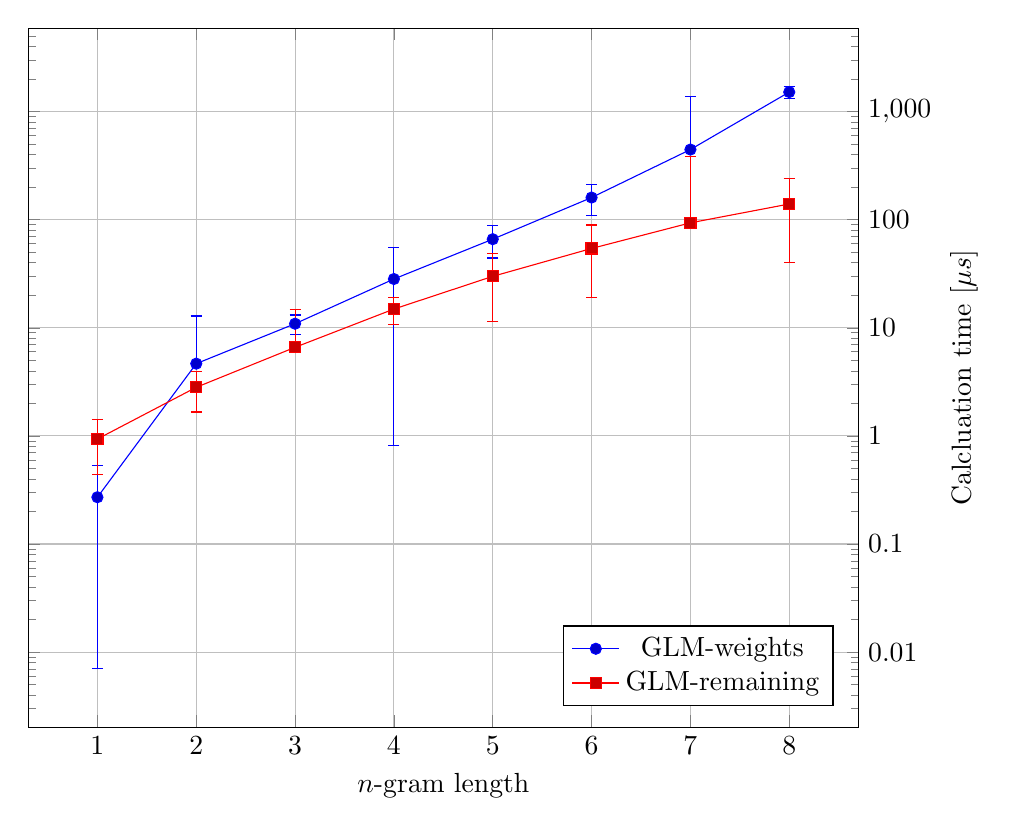
\begin{tikzpicture}[baseline]

\begin{axis}[
  xlabel = {$n$-gram length},
  xtick = {1, ..., 8},
  ylabel = {Calcluation time [$\mu s$]},
  yticklabel pos = right,
  ymode = log,
  log ticks with fixed point,
  %yticklabel pos = right,
  minor y tick num = 4,
  grid = major,
  legend entries = {{GLM-weights}, {GLM-remaining}},
  legend pos = south east,
  width = \textwidth,
]

% GLM-weights
\addplot+[
  error bars/.cd,
  y dir = both,
  y explicit,
] table [y error = us_error] {
  n  us        us_error
  1     0.271    0.264
  2     4.659    8.199
  3    10.904    2.241
  4    28.258   27.442
  5    65.981   21.772
  6   160.189   51.710
  7   445.098  923.704
  8  1513.286  192.037
};

% GLM-remaining
\addplot+[
  error bars/.cd,
  y dir = both,
  y explicit,
] table [y error = us_error] {
  n  us        us_error
  1     0.936    0.494
  2     2.815    1.151
  3     6.599    8.195
  4    14.907    4.238
  5    29.901   18.446
  6    54.152   35.138
  7    93.452  291.793
  8   139.598   99.582
};

\end{axis}

\end{tikzpicture}
\end{document}
